\documentclass{beamer}
\usepackage{lsfolien}
\usepackage[english]{babel}
\usepackage[utf8]{inputenc}

\myfootline{System Modelling and Semantic Web -- Winter Term 2021}{Hans-Gert
  Gräbe} 

\newcommand{\ueberschrift}[1]{\begin{center}\bf #1\end{center}}

\title{Modelling Sustainable Systems\\ and Semantic Web\\[6pt]
  Systems and their Development
  \vskip1em}

\subtitle{Lecture in the Module 10-202-2309\\ for Master Computer Science}

\author{Prof. Dr. Hans-Gert Gräbe\\
\url{http://www.informatik.uni-leipzig.de/~graebe}}

\date{October 2021}
\begin{document}

{\setbeamertemplate{footline}{}
\begin{frame}
  \titlepage
\end{frame}}

\begin{frame}{What is a System?}
Summary of the previous lecture and the seminar on Tuesday.

  \begin{block}{System definition}
    A \emph{system} is a \emph{delimited set of components}.  Their
    interaction realises a \emph{qualitatively new function} (emergent
    function) and thus constitutes \emph{a new unified whole}.
  \end{block}

The systemic approach is a form of reduction of the complexity of the totally
interconnected real-world (\emph{reality} for short).
\end{frame}

\begin{frame}{What is a System?}
  \begin{block}{Three dimensions of reduction to the essentials.}
    \begin{itemize}
    \item[(1)] Outer demarcation of the system against an \emph{environment},
      reduction of these relationships to input/output relationships
      (specifications and interfaces) and guaranteed throughput.
    \item[(2)] Inner demarcation of the system by combining subareas to
      \emph{components}, whose functioning is reduced to “behavioural control”
      via input/output relations (specifications and interfaces).
    \item[(3)] Reduction of the relations in the system itself to “causally
      essential” relationships.
    \end{itemize}
  \end{block}
\end{frame}

\begin{frame}{What is a System?}
This reduction is essential for both the \emph{description} of real-world
contexts and for their \emph{operational control}.

In this understanding, systems are to be considered as a \textbf{unit of
  analysis/description (modelling) and execution (operation)}, emphasising the
\emph{structuredness} and thus \emph{decomposability} of the system in the
analytic dimension on the one hand, and the \emph{interdependence} and thus
\emph{indecomposability} in the operational dimension on the other.

In the assembled system in addition to the components, the \emph{connecting
  elements} also play an important role.  They mediate the \emph{flow of
  energy, material and information} that is required for the operation of each
component.
\end{frame}

\begin{frame}{Systems and the Theory of Dynamical Systems}

  The Theory of Dynamical Systems is an important mathematical description
  tool for the operational dimension of the system model used to
  \emph{quantify its laws of motion}.

  In the simplest case (Seminar on Tuesday), the elements of such a dynamical
  system are atomic. In the general case, the parts (components) of the
  dynamical system come with their own dynamics, which are combined to form
  the dynamics of the overall system.

  As reduction to essentials takes place, the dynamics of the components do
  \textbf{not} enter with their full complexity into the modelling of the
  overall system.
\end{frame}

\begin{frame}{Systems and Practice}
Systems are a part of the complex relationships of practice.

Analysis and modelling as human thinking activities not only have a
\emph{mental quality}, but also a \emph{practical} one. The goal of modelling
is to influence real-world processes; the \emph{criterion of "truth"} is
formed from practical experience, how successful the mental modelling and
\emph{intended transformation of the real-world substrate} are related.

However, this experience itself can only be communicated intersubjectively in
language form and is thus itself of mental quality.

A coherent concept of a system must combine both dimensions -- logos and
telos.
\end{frame}

\begin{frame}{Systems and Autonomy}
The concept of system in such a version suggests a certain \emph{autonomy of
  systems}.

On the other hand, the system concept is self-similar -- components can again
be considered and analysed as systems.

However, this is done under a \emph{different reduction to essentials} than
for the overall system.

In such an understanding, components are part of an overall system in which
the component dynamics influence each other and thereby \emph{jointly produce
  the emergent function of new quality} of the overall system. This undermines
the notion of autonomy (of the components as systems in their own).

Closed and Open Systems.   
\end{frame}

\begin{frame}{Open Systems}
Open systems can be modelled like closed ones if a qualitatively and
quantitatively determined \textbf{throughput of energy, matter and
  information} is additionally postulated.

\begin{block}{Altshuller's Law of Energy Conductivity.}
  A necessary condition for the viability of a technical system is the flow of
  energy through all its parts.
\end{block}

This external throughput is often constitutive for the inner system structure
through resonance and dissonance phenomena of amplification and extinction of
inner dynamics.

\begin{block}{Altshuller's Law of Coordination of the Rhythm of the Parts.}
  A necessary condition for the viability of a technical system is the
  coordination of the rhythms of all parts of the system.
\end{block}
\end{frame}

\begin{frame}{Change the World as Planned}
The system concept is a tool in the hands of humans who want to \textbf{change
  the world} following their (intentions, goals and) plans.

\begin{block}{11th Feuerbach Thesis (Marx)}
  Philosophers have only interpreted the world differently, it is a matter of
  changing it.\\[4pt] Die Philosophen haben die Welt nur verschieden
  interpretiert, es kömmt darauf an, sie zu verändern.
\end{block}

But: The world is in constant motion and also permanently changes itself.

So more precisely: It is a matter of \textbf{influencing the development of
  reality}.
\end{frame}

\begin{frame}{Modelling Systems}

Two practical tasks:
\begin{itemize}
\item[(1)] Build new system
\item[(2)] Rebuild existing system
\end{itemize}

(1) can be consideres as a special case of (2), since every need for a new
system comes with at least rough ideas about that new system, so there is also
under (1) an at least rough description form of the system to be created.

\begin{center}
  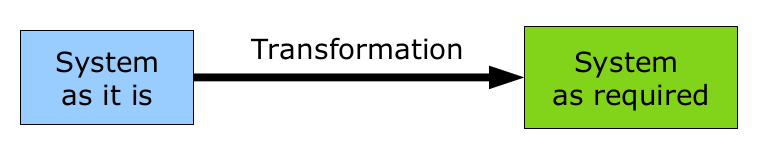
\includegraphics[width=.9\textwidth]{Bilder/SD-1.png}
\end{center}
\end{frame}

\begin{frame}{Modelling Systems}
  This basic scheme fits not only technical systems, but also the modelling of
  social, socio-ecological and cultural systems, so it is sufficiently
  universal.

How does such a system evolve over time?
\begin{center}
  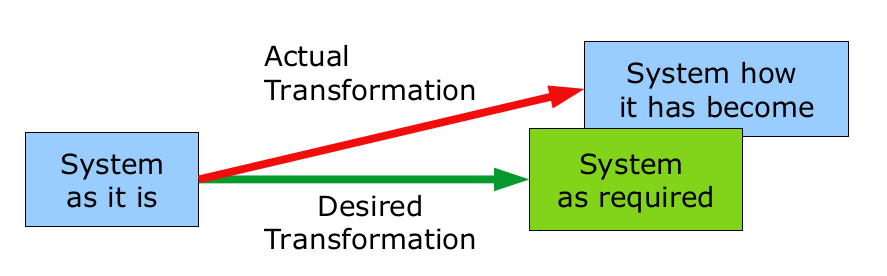
\includegraphics[width=.9\textwidth]{Bilder/SD-2.png}
\end{center}
\end{frame}

\begin{frame}{Development of Systems}
\begin{center}
  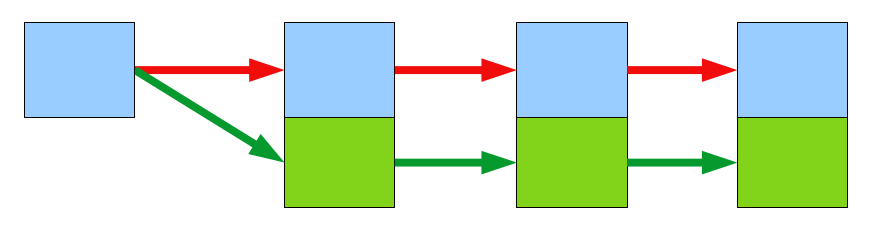
\includegraphics[width=.9\textwidth]{Bilder/SD-3.png}
\end{center}
Transitional development as \emph{different versions} of the system over the
time.
\end{frame}

\begin{frame}{Development of Systems}
  \begin{minipage}{.45\textwidth}
    But this can also be understood as development in time \emph{of the same
      system}.\vskip1em

    Transitional management versus adaptive management.
  \end{minipage}\hfill
  \begin{minipage}{.45\textwidth}
    \begin{center}
      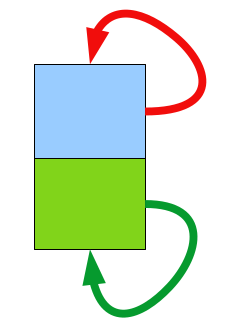
\includegraphics[width=.6\textwidth]{Bilder/SD-4.png}
    \end{center}
  \end{minipage}
\end{frame}

\begin{frame}{Development of Systems}
  The development of a system can therefore be conceived as a contradiction
  between an \emph{ideal line of development} and a \emph{real line of
    development}.

This idea is reflected in the \textbf{TRIZ concept of the \emph{Ideal Final
    Result}} (IFR -- Ideales Endresultat).

In the Theory of Dynamical Systems, system development is conceived as a
progression of states, which can be described by a function $f(t)$ with values
in a phase space.

The \emph{ideal behaviour} is described by mathematical relationships, such as
differential equations of the laws of motion and geometrically displayed as
\emph{trajectory}. 

\end{frame}

\begin{frame}{System Dynamics}
These differential equations and trajectories are part of the
\emph{description form of the system} and thus have already been created by
\emph{reduction to essentials}.

In the modelling it is assumed that everything essential is taken into
account, i.e. that the \emph{real temporal development} $r(t)$ of the system
differs from the \emph{ideal temporal development} $f(t)$ only by a small
difference $d(t)=r(t)-f(t)$, which is \emph{insignificant for the selected
  essential}.

While $f(t)$ enables a \emph{quantitative prediction} of the development of
the system, the statement that $d(t)$ is "small" or "damped" is a
\emph{qualitative statement} of the description form itself.

\end{frame}

\begin{frame}{System Dynamics}
Often one also restricts oneself with $f(t)$ to a \emph{qualitative statement}
about the exact position of the trajectories as invariants in the solution
space and thus to the statement that $r(t)$ oscillates around these
trajectories in a damped manner.  These trajectories seem to "magically"
attract the real states and are therefore also called \emph{attractors}
(steady state equilibrium).

For example, the Earth moves on an elliptical orbit around the Sun in the
sense that real deviations from this orbit are compensated.

\end{frame}

\begin{frame}{Coevolution of Systems}
\begin{minipage}{.55\textwidth}
  What is the relationship between the development
  \begin{itemize}
  \item of the system itself,
  \item of the components in the system and
  \item of the relationships in the system?
  \end{itemize}
\end{minipage}\hfill 
\begin{minipage}{.4\textwidth}
    \begin{center}
      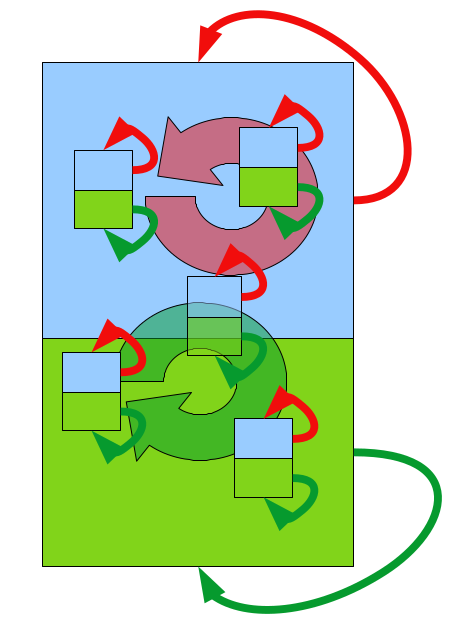
\includegraphics[width=.95\textwidth]{Bilder/SD-5.png}
    \end{center}
  \end{minipage}
\end{frame}

\begin{frame}{Coevolution of Systems}

The coupling of developments between components is driven by resonance
phenomena and coupled to eigentimes and eigenspaces of the inner equations of
motion, different for different components.\vskip2em

\begin{block}{Altshuller's Law of Non-uniformity of the Development of the
    Parts of a System.}  The parts of a system develop non-uniformly; the more
  complicated the system, the more non-uniformly develop its parts.
\end{block}
\end{frame}

\end{document}
